\documentclass{article}
\usepackage[lyric]{songs}
\usepackage{graphicx}
\usepackage{pdfpages}
\graphicspath{ {./images/} }

\newindex{index}{idxfile}
    

\nosongnumbers

 
\begin{document}
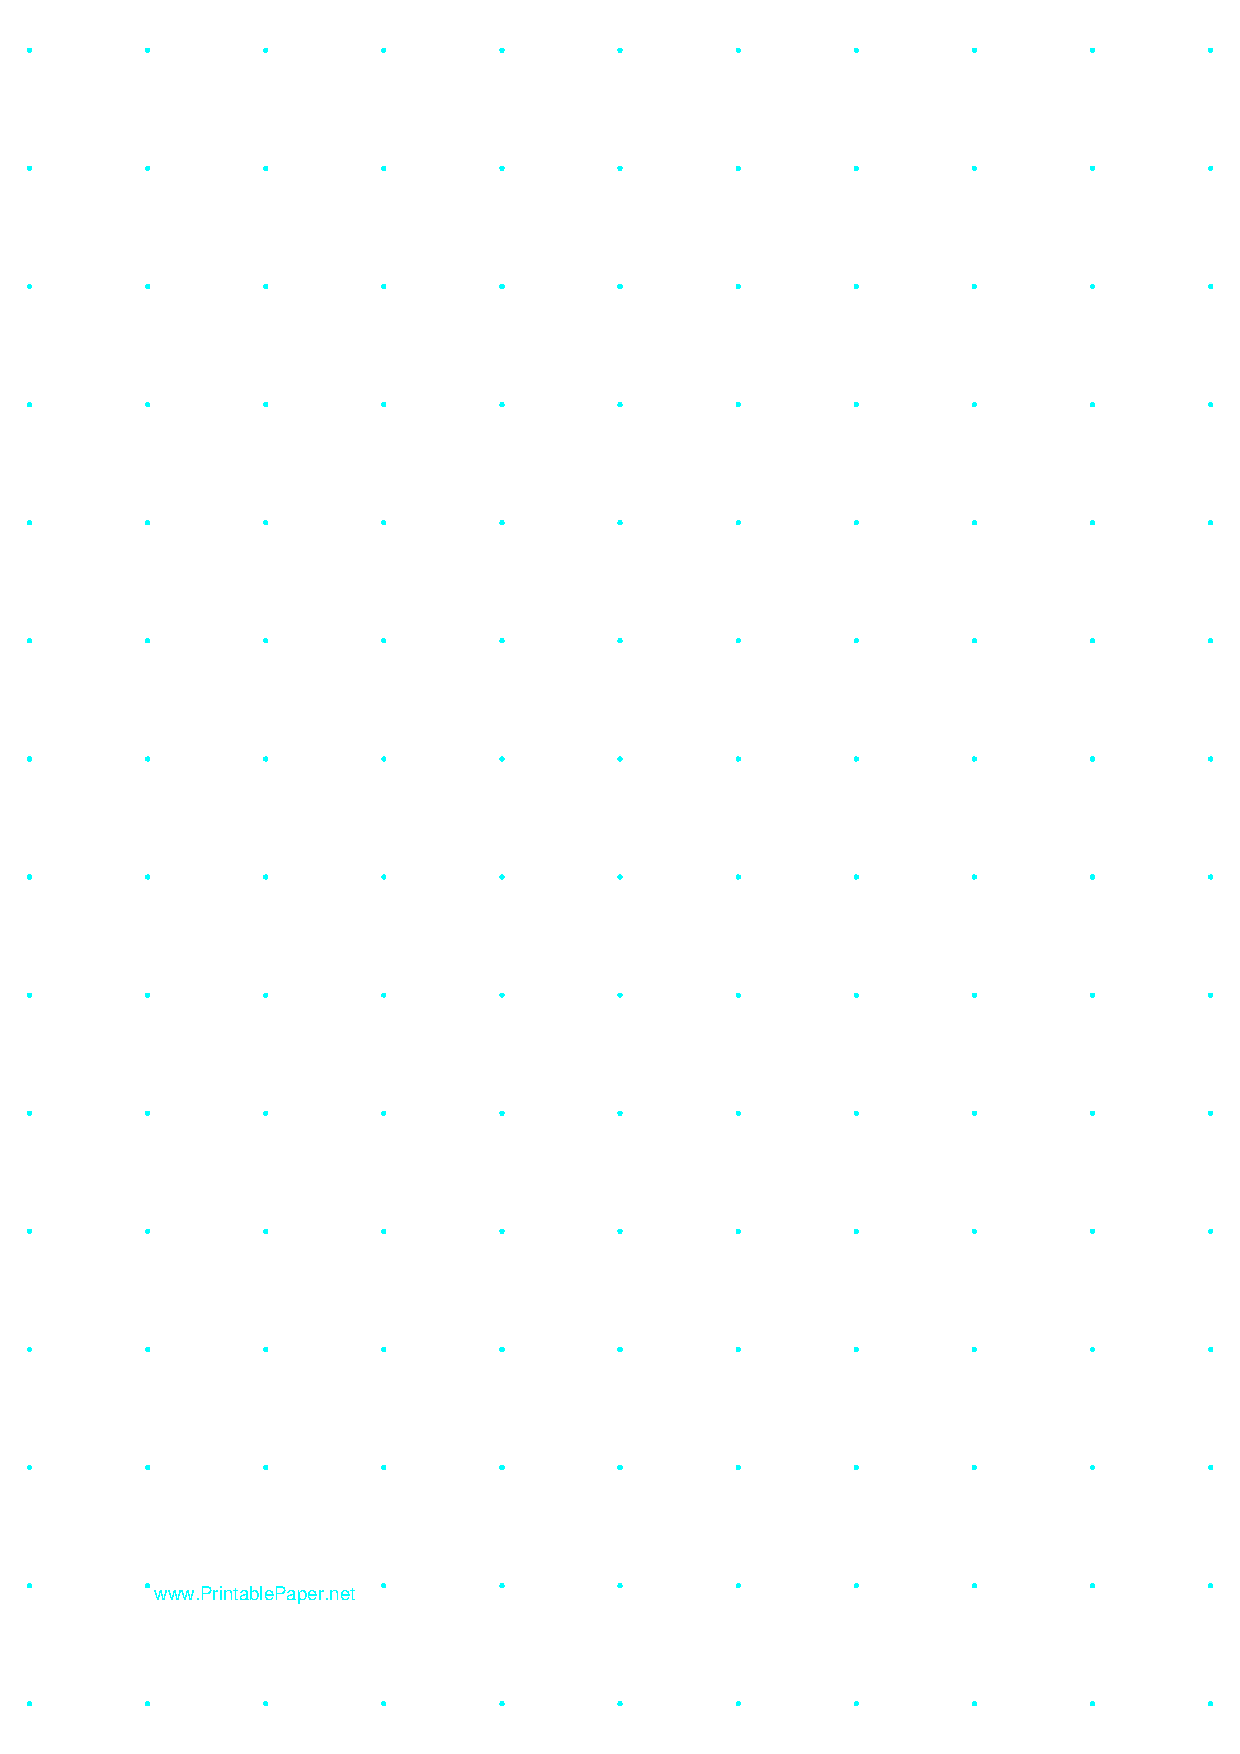
\includepdf{voorblad.pdf}    
\begin{songs}{}
\beginsong{'k Heb mijn wagen volgeladen}
\beginverse*
'k Heb mijn wagen volgeladen,
Vol met oude wijven;
Toen ze op de marrekt kwamen,
Begonnen zij te kijven
Nu neem ik van mijn levensdagen
Geen oude wijven meer op mijn wagen!
Hop, paardje hop!
\endverse
\beginverse*
'k Heb mijn wagen volgeladen,
Vol met oude mannen
Toen zij op de marrekt kwamen,
Gingen ze samenspannen.
Nu neem ik van mijn levensdagen
Geen oude mannen meer op mijn wagen!
Hop, paardje hop!
\endverse
\beginverse*
'k Heb mijn wagen volgeladen,
Vol met jonge meisjes
Toen zij op de marrekt kwamen,
Zongen zij als sijsjes
Nu neem ik van mijn levensdagen
Steeds jonge meisjes op mijn wagen!
Hop, paardje hop!
\endverse
\endsong
\begin{intersong}
    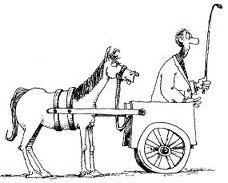
\includegraphics[width=0.4\textwidth]{img1}
\end{intersong}
\beginsong{'s Monjdoos}
\beginverse*
En 's monjdoos, tein gommen nie weirken.
En tauësjendoos gommen op zwier.
Goensjtoogs zeu zat as e veirken.
En tonderdoos spauve me zier.
Tvrauëdoos, tein gommen beginnen.
En sooëterdoos emmen geen pree.
Wa moet er ons vrauken beginnen,
me azeu ne zatte kadee?
\endverse
\beginverse*
Drinkt, drinkt, drinkt aujlen zat,
drinkt aujlen e stik in a kleuten.
Drinkt, drinkt, drinkt aujlen zat,
drinkt aujlen e stik in a gat.
\endverse
\endsong
\beginsong{'t Is welle, welle, wel}
\beginverse*
‘t Is welle, welle, wel, ‘t is wel
‘t Is welle, welle, wel, ‘t is wel
‘t Is welle, welle, wel,
‘t Is zeker wel,
‘t Is welle, welle, wel, ‘t is wel
\endverse
\endsong
\beginsong{A la claire Fontaine}
\beginverse
A la claire Fontaine
M'en allant promener,
J'ai trouvé l'eau si belle
Que je m'y suis baigné.
\endverse
\beginchorus
Il y a longtemps que je t'aime
jamais je ne t'oublierai …
\endchorus
\beginverse
Sous les feuilles d'un chêne
Je me suis fait sécher
Sur la plus haute branche
Le rossignol chantait
\endverse
\beginverse
Chante rossignol, chante
Toi qui as le coeur gai;
Tu as le coeur à rire
Moi je l'ai à pleurer.
\endverse
\beginverse
J'ai perdu mon amie
Sans l'avoir mérité
Pour un bouquet de roses
Que je lui refusai
\endverse
\beginverse
Je voudrais que la rose
Fût encore à planter
Et que ma douce amie
Fut encore à m'aimer
\endverse
\endsong
\beginsong{A ram sam sam}
\beginverse*
A ram sam sam, a ram sam sam
Goeli goeli goeli goeli
ram sam sam
Arabi , Arabi
Goeli goeli goeli goeli
ram sam sam.
\endverse
\endsong
\beginsong{Ahoelaba}
\beginverse
In d' Afrikaanse bossen, waar alle negers krossen.
Daar in die wildernis, daar woont mijn Oela Oelaba.
\endverse
\beginchorus
Ahoelaba, ik van je hou.
Ahoelaba, jij wordt mijn Afrikaanse vrouw.
\endchorus
\beginverse
Ik bloemen pluk voor Oela, maar Oela ze verkoop.
Ik Oela kusje geven, en Oela aan de loop.
\endverse
\endsong
\begin{intersong}
    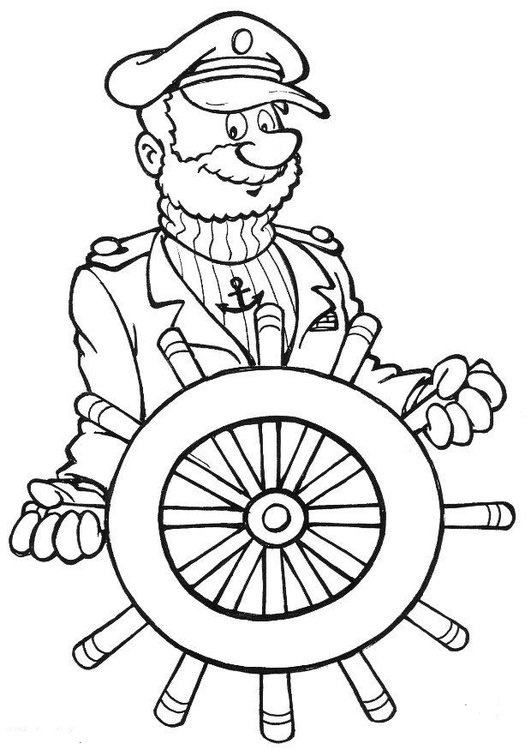
\includegraphics[width=0.4\textwidth]{img2}
\end{intersong}
\beginsong{Al die willen te kaap'ren  varen}
\beginverse*
Al die willen te kaap'ren  varen, moeten mannen met baarden zijn.
Jan, Piet, Tjores en Corneel: Die hebben baarden, die hebben baarden.
Jan, Piet, Tjores en Corneel: Die hebben baarden, zij varen mee.
\endverse
\endsong

\beginsong{Aloutte}
\beginverse
Alouette, gentille alouette, alouette, je te plumerai.
Je te plumerai la tete. 
Je te plumerai la tete et la tete.
O, alouette gentille alouette, alouette, je te plumerai.
\endverse
\beginverse
Alouette, gentille alouette, alouette, je te plumerai.
Je te plumerai le bec.
Je te plumerai le bec et le bec et la tete.
O, alouette, gentille alouette, alouette, je te plumerai.
\endverse
\beginverse
...le ne'z...et le bee...et la tete
\endverse
\beginverse
...le dos...et le nez...etc...
\endverse
\beginverse
...les pattes...et le dos...etc...
\endverse
\beginverse
 ...le cou...et les pattes...etc...
\endverse
\endsong
\beginsong{Des winters als het regent}
\beginverse
Des winters als het regent, dan zijn de paadjes diep, ja diep.
Dan komt dat loze vissertje, vissen al in dat riet, ja riet.
\endverse
\beginchorus
Met zijnen rijfstok, met zijnen strijkstok.
Met zijnen lapzak, met zijnen knapzak.
Met zijnen lere, van dirre domme dere.
Met zijne lere laarsjes aan. 
\rep{2}
\endchorus
\beginverse
Dat loze molenarinnetje, hing in heur deurtje staan, ja staan.
Opdat dat aardig vissertje, voorbij haar heen zou gaan, ja gaan.
\endverse
\beginverse
Wat heb ik u misdreven? Wat heb ik u misdaan, ja 'daan.
Opdat ik niet met vrede, vorbij uw deur mag gaan, ja gaan
\endverse
\beginverse
Gij hebt mij niets misdreven, gij hebt mij niets misdaan, ja 'daan.
Maar moet mij driemaal zoenen, eer gij van hier moogt gaan, ja gaan.
\endverse
\beginchorus
Met uwen rijfstok, met uwen strijkstok.
Met uwen lapzak, met uwen knapzak.
Met uwen lere, van dirre domme dere.
Met uwe lere laarsjes aan. 
\rep{2}
\endchorus
\endsong
\beginsong{Als de djungel}
\beginverse*
Als de djungel zich hult in het duister, flauw verlicht door het schijnsel der maan.
Sta dan stil, spits je oren en luister, zwijgend zie je de horde daar staan. 
\endverse
\beginchorus
Jalahi weerklinkt door de rimboe, 't is de kreet van het hoofd van de stam.
Alle wolven, Bagheera en Baloe, hurken neer bij de laaiende vlam. 
(En nog ne keer!)
\endchorus
\endsong
\begin{intersong}
    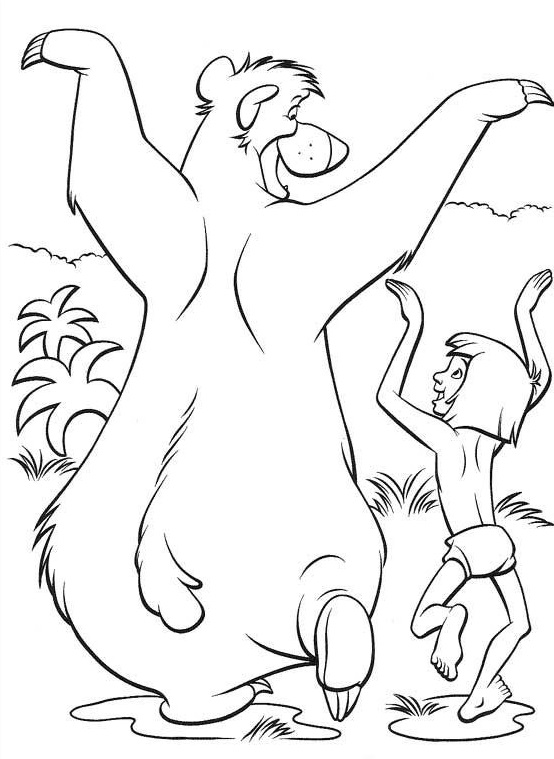
\includegraphics[width=0.4\textwidth]{img3}
\end{intersong}
\beginsong{Als de rombom}
\beginverse
Als de rombom heeft geslagen, en wij marcheren moeten gaan, geweer en ransel die moeten wij dan dragen, en dat staat ons voorwaar niet aan. 
\endverse
\beginchorus
Kapiteins en officieren, drinken wijn en soms een glaasje bier maar wij zijn maar arme fuselieren, drinken water al uit de rivier.
\endchorus
\beginverse
Een stuiver daags is onze gage, en een pondje zwart kommiezenbrood, een watersausje dat geeft ons de courage, en daarmee moeten wij dan maar voort.
\endverse
\endsong
\beginsong{Als in de mei}
\beginverse
Als in de mei, de blijde mei,
de merel fluit in 't woud,
ja fluit in 't woud,
dan trekken jonge kerels, 
van niets benauwd,
dan trekken jonge kerels, 
van niets benauwd.
\endverse
\beginchorus
Juvi valle valle valle valle lala
Juvi valle valle valle valle lala
Dan trekken jonge kerels, 
van niets benauwd.
\endchorus
\beginverse
Zij zingen luid hun lustig lied,
dat 't galme door het woud, 
ja door het woud.
Ze stappen 't leven tegen, 
van niets benauwd,
ze stappen 't leven tegen, 
van niets benauwd.
\endverse
\beginverse
Ach fiere jeugd, ach fiere jeugd,
uw lied klinkt veel te stout, 
ja veel te stout.
Ge zult wel anders zingen,
wordt gij eens oud,
Ge zult wel anders zingen,
wordt gij eens oud.
\endverse
\beginverse
Wij zingen nooit een ander lied,
al klinkt het nog zo stout,
ja nog zo stout.
Wij stoere vlaamse kerels, 
nooit worden w' oud,
wij stoere vlaamse kerels, 
nooit worden w' oud.
\endverse
\endsong
\begin{intersong}
    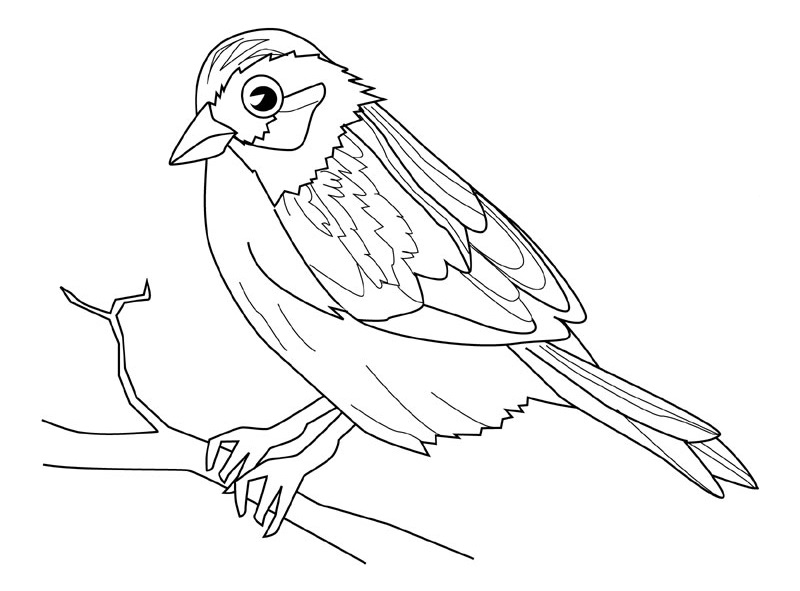
\includegraphics[width=0.4\textwidth]{img4}
\end{intersong}
\beginsong{Anne mie}
\beginverse*
Anne mie, warum hast du mir nicht geschrieben?
Anne mie, warum hast du mir nicht geschrieben?
Anne mie, und ich vergess dich nie.
Ich mag so gern, so gern nach House wiedergehn, und meine Liebste wiedersehen.
Ich mag so gern, so gern nach House wiedergehn, und meine Liebste wiedersehen.
\endverse
\beginverse*
Infanterie, du bist der schönste aller Waffen.
Infanterie, du bist der schönste aller Waffen.
Infanterie, und ich vergess dich nie...
\endverse
\endsong
\beginsong{Annemarieken}
\beginverse*
Wel Annemarieken waar ga je naartoe? \rep{2}
'k Ga naar den buiten al bij de soldaten hopsasafallala Annemarie. \rep{2}
\endverse
\beginverse*
Wel Annemarieken wat ga je daar doen? \rep{2}
Haspen en spinnen, soldaatjes beminnen hopsasafallala Annemarie. \rep{2}
\endverse
\beginverse*
Wel Annemarieken heb jij er geen man? \rep{2}
Heb ik geen man, dan krijg ik geen slagen hopsasafallala Annemarie. \rep{2}
\endverse
\beginverse*
Wel Annemarieken heb jij er geen kind? \rep{2}
Heb ik geen kind, dan moet ik niet zorgen hopsasafallala Annemarie. \rep{2}
\endverse
\endsong
\beginsong{Au clair de la lune}
\beginverse*
Au clair de la lune, mon ami Pierrot. Prete-moi ta plume pour ecrire un mot. Ma chandelle est morte, je n'ai plus de feu, ourvre-moi ta porte pour l'amour de Dieu!
\endverse
\beginverse*
Au clair de la lune,Pierrot repondit: "Je n'ai pas de plume, Je suis dans mon lit. Va chez la voisine, Je crois qu'ell y est, car dans sa cuisine on bat le briquet."
\endverse
\beginverse*
Au clair de la lune, L'aimable Lubin. Frappe chew la brune, Ell' repond soudain: "Qui frappe d'la sorte?" Il dit a son tour: "Ouvrez votre porte pour le dieu d'amour!"
\endverse
\beginverse*
Au clair de la lune, On n'y voit qu'un peu. On chercha la plume, On chercha du feu. En chercant d'la sort, Je n'sais c' qu'on trouva: Mais j'sais que la porte  sur eux se ferma.
\endverse
\endsong
\begin{intersong}
    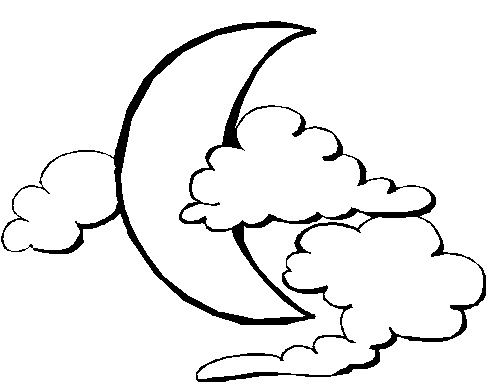
\includegraphics[width=0.4\textwidth]{img5}
\end{intersong}
\beginsong{Auprès de ma blonde}
\beginverse
Dans les jardins d'mon père, les lilas sont fleuris, tous les oiseaux du monde y viennent faire leur nid.
\endverse
\beginchorus
Auprès de ma blonde, qu'il fait bon, fait bon, fait bon.
Auprès de ma blonde, qu'il fait bon dormir.
\endchorus
\beginverse
Tous les oiseaux du monde y viennent faire leur nid, la caille, la tourtelle, et la jolie perdrix.
\endverse
\beginverse
La caille, la tourtelle, et la jolie perdrix, et ma jolie colombe, qui chante jour et nuit.
\endverse
\beginverse
Et ma jolie colombe, qui chante jour et nuit, qui chante pour les filles, qui n’ont point de mari.
\endverse
\beginverse
Qui chante pour les filles, qui n’ont point de mari, pour moi ne chante guère, car j’en ai un jolie.
\endverse
\beginverse
Pour moi ne chante guère, car j’en ai un jolie, dites-nous, donc, la belle, ou donc est votr’mari.
\endverse
\beginverse
Dites-nous, donc, la belle, ou donc est votr’mari, il est dan la Holland, les Hollandais l’ont pris.
\endverse
\beginverse
Il est dan la Hollande, les Hollandais l’ont pris, que donneriez-vous, belle, pour avoir vort’mari
\endverse
\beginverse
Qui donneriez-vous, belle, pour avoir votr’mari, je donnerais Versailles, Paris et Saint-Denis.
\endverse
\beginverse
Je donnerais Versaille, Paris et Saint-Denis, les tours de Notre-Dame et l’clocher de sons pays.
\endverse
\beginverse
Les tours de Notre-Dame et l’clocher de sons pays, et ma joli colombe, pour avoir mon ami.
\endverse
\endsong
\beginsong{Avondlied}
\beginverse
O Heer, d'avond is neergekomen. De zonne zonk, het duister klom. De winden doorruisen de bomen. En verre sterren staan alom. Wij knielen neer om U te zingen. In't slapend woud ons avondlied. Wij danken U voor wat we ontvingen. En vragen, Heer, verlaat ons niet.
\endverse
\beginchorus
Scouts en leiders knielen wij neder. Door de stilte weerklinkt onze bee. Luistrend fluistren kruinen mee. En sterren staren teder. Geef ons, Heer, zegen en rust en vree...
\endchorus
\beginverse
Gij hebt dezen dag ons gegeven. En ons bewaard gezond en blij. Uw engel is ons bijgebleven. En heeft gewandeld aan ons zij! We deden goed met uw genaden. We leerden menig wijze raad. Eenieder heeft door woord en daden. Zijn makkers broederlijk gebaat!
\endverse
\beginverse
Al wat wij boos en zwak misdeden. Vergeef het ons, O goede Heer. Uw liefde heeft voor ons geleden. Wees ons barmhartig nog een keer... Wij willen weer U trouw beloven. Ons Woord vernieuwen, Heer, voor U. En zeker van Uw hulp van boven. Laat ons gelukkig slapen nu!
\endverse
\beginverse
Weleer toen uw apostlen sliepen, toen badt G'op enen berg alleen. Waak over ons, die U aanriepen. Drijf duivel, dood en vijand heen... Waak over ons, Gij, Licht en Leven, Gij Waarheid, en 'ge Levensbaan. En morgen wordt U weer gegeven, Elke avond, ieder zonopstaan!
\endverse
\endsong
\begin{intersong}
    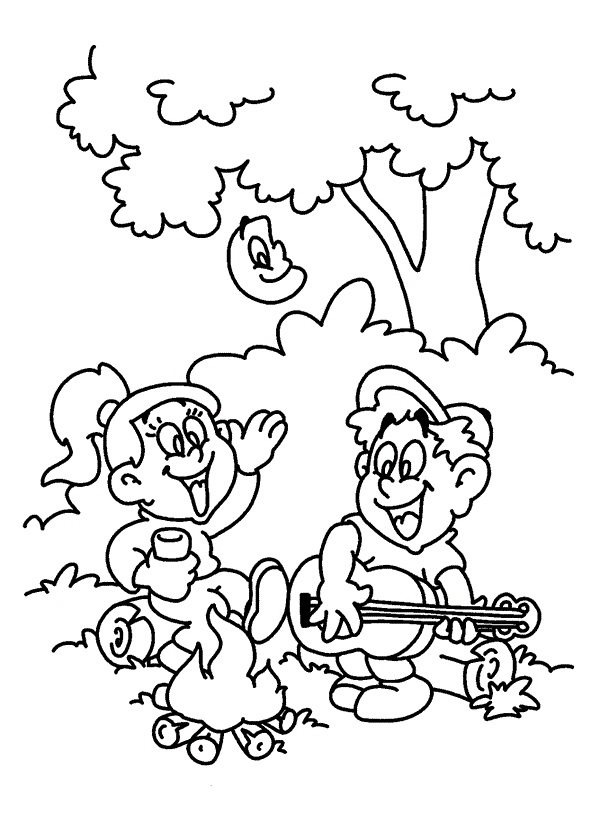
\includegraphics[width=0.4\textwidth]{img6}
\end{intersong}
\beginsong{Begroetingslied}
\beginverse*
hallo, hallo, hallo , hallo
Wij komen u groeten
Zijn blij u t'ontmoeten
hallo, hallo, hallo , hallo
\endverse
\endsong
\beginsong{Belgisch Volkslied}
\beginverse*
O dierbaar Belgie, O heilig land der vad'ren, Onze ziel en ons hart zij U gewijd.
Aanvaard ons kracht en het bloed van ons ad'ren. Wees ons doel in arbeid en in strijd.
Bloei o land, in eendracht niet te breken. Wees immer uzelf, en ongeknecht.
Het woord getrouw dat ge onbevreesd moogt spreken: Voor vorst, voor vrijheid en voor recht.
Voor vorst, voor vrijheid en voor recht.\rep{2}

\endverse
\endsong
\beginsong{Beloftelied}
\beginverse
Wij hebben u, o Jezus
Plechtig beloofd
U altijd te erkennen
Als opperhoofd.
\endverse
\beginchorus
Geef dat w'u minnen zouden
Steeds meer en meer,
Help ons belofte houden
Jezus onze Heer.
\endchorus
\beginverse
Wij hebben het gezworen
Dat Gij steeds zoudt
Ons hoofd en leider wezen
Als opperscout.
\endverse
\beginverse
Geef dat w'u minnen zouden
Steeds meer en meer,
Help ons belofte houden
Jezus onze Heer.
\endverse
\beginverse
Wij zullen gans ons leven
Lijk Gij 't geboodt
U volgen en U dienen
Tot aan ons dood.
\endverse
\beginverse
Geef dat w'u minnen zouden
Steeds meer en meer,
Help ons belofte houden
Jezus onze Heer.
\endverse
\endsong
\beginsong{Bergvagebunden}
\beginverse
Wenn wir erklimmen schwindelnde Höhen,
Steigen dem Gipfelkreuz zu;
In unsern Herzen brennt eine Seesicht,
Die lässt uns nimmer mehr in ruh. 
\endverse
\beginchorus
Herrliche Berge, Sonnige Höhen,
Bergvagebunden sind wir, ja wir,
Herrliche Berge, Sonnige Höhen,
Bergvagebunden sind wir.
\endchorus
\beginverse
Mit Seil und Haken, den Tod im Nacken,
Hängen wir an der steilen Wand. 
Herzen erglühen, Edelweiß blühen,
Vorbei geht’s mit sicheren Hand.
\endverse
\beginverse
La Montanara und Puchiana,
Berge sind überall schön.
Gletscher und Sonne, Herzen voll Wonne,
Herllich die Berge zu sehn.
\endverse
\beginverse
Beim Alpenglühen heimwärts wir ziehen,
Berge, die leuchten so rot. 
Wir kommen wieder, denn wir sind Brüder,
Brüder auf Leben und Tod.
\endverse
\beginchorus
Lebwohl ihr Berge,
Sonnige Höhen,
Bergvagebunden sind treu, ja treu,
Lebwohl ihr Berge, Sonnige Höhen,
Bergvagebunden sind treu. 
\endchorus
\endsong
\beginsong{Bert Rodenbach}
\beginverse*
Bert Rodenbach die heeft een vogel in zijn hand. 
Bert Rodenbach die heeft een vogel in zijn hand.
Bert Rodenbach die heeft een vogel in zijn hand, een vogel in zijn hand. Tarara…
\endverse
\beginverse
Bert Rodenbach die heeft een vogel in zijn …
\endverse
\beginverse
Bert Rodenbach die heeft een vogel in …
\endverse
\beginverse
Bert Rodenbach die heeft een vogel …
\endverse
\beginverse
Bert Rodenbach die heeft een …
\endverse
\beginverse
Bert Rodenbach die heeft ...
\endverse
\beginverse
Bert Rodenbach die …
\endverse
\beginverse
Bert Rodenbach …
\endverse
\beginverse
Bert ...
\endverse
\endsong
\beginsong{Bier her, Bier her}
\beginverse*
Bier her, Ber her, 
oder ich fall’um jochhe,
Bier her, Bier her,
oder ich fall’um.
Soll das BIer im Keller liegen,
und ich hier die ohnmacht kriegen,
Bier her, Bier her,
oder ich fall’um.
\endverse
\beginverse*
Bier her, Bier her,
oder ich fall’um jochhe,
Bier her, Bier her,
oder ich fall’um.
Wenn nicht gleich Bier bekumm’
schmeisz’ich ganze Kneipe um.
Bier her , Bier her,
oder ich fall’um.
\endverse
\endsong
\beginsong{Blowing in the wind}
\beginverse
How many roads must a man walk down
Before they call him a man?
How many seas must a white dove sail
Before she sleeps in the sand?
How many times must the cannonballs fly
Before they're for ever band?
\endverse
\beginchorus
The answer my friend,
Is blowin' in the wind,
The answer is blowin' in the wind.
\endchorus
\beginverse
How many times must a man look up
Before he can see the sky?
How many ears must one have
Before he can heare people cry?
How many deaths will it take till he know
That to many people had died?
\endverse
\beginverse
How many years can a mountain exist
Before he washed to the sea?
How many years can some people exist
Before they're allowed to be free?
How many times can a man turn his head
And pretend that he just doesn't see?
\endverse
\endsong
\beginsong{Brede velden}
\beginverse*
Brede velden, verre heiden,
waar ons hart zicht aan verpandt.
In uw stille, trouwe aarde,
staat zo menig kruis geplant.
In uw stille, trouwe aarde,
staat zo menig kruis geplant.
\endverse
\beginverse*
Oude fierheid, lang vergeten,
hoe lang nog blijft gij geknecht?
In ons harten, kameraden,
brandt ‘t vuur dat land weer recht.
In ons harten, kameraden,
brandt ‘t vuur dat land weer recht.
\endverse
\endsong
\beginsong{Chevaliers de la table ronde}
\beginverse
Chevaliers de la table ronde,
allons voir si le vin est bon
\endverse
\beginchorus
Allons voir, oui, oui, oui,
allons voir, non , non, non,
allons voir, si le vin est bon.
\endchorus
\beginverse
J’en boira cinq à six bouteilles,
une femme sur mes genoux.
Mais voilà qu’on frappe à la porte
je crois bien que c’est le mari.
\endverse
\beginverse
Si je meurs, je veux qu’on m’enterre,
dans une cave où il y a du bon vin.
Les deux pieds contre la muraille,
et la tête sous le robinet.
\endverse
\beginverse
Sur ma tombe je veux qu’on inscrive:
ici gît le roi des buveurs.
La morale de cette histoire,
c’est de boire avant de mourir.
\endverse
\beginverse
La morale de cette morale
c’est que les hommes sont des couchons
La morale de cette morale
c’est que les femmes aiment les couchons.
\endverse
\endsong
\beginsong{Clementine}
\beginverse
In a cavern, in a canyon,
excavating for a mine,
dwelt a miner, fortyniner, 
and his daughter, Clementine.
\endverse
\beginchorus
Oh my darling, oh my darling,
oh my darling, Clementine.
You are lost and gone forever,
dreadful sorry, Clementine.
\endchorus
\beginverse
Light she was, and like a fairy,
and her shoes were number nine,
Herring boxes, without topses,
sandals were for Clementine.
\endverse
\beginverse
Drove she ducklings to the water,
ev’ry morning, just at nine
hit her foot against a splinter,
fel into the foaming brine.
\endverse
\beginverse
Ruby lips above the water,
blowing bubbles, soft and fine,
but alas, I was no swimmer, 
so I lost my clementine.
\endverse
\beginverse
When the miner forty-niner,
Soon began to peak and pine,
Thought he oughter "jine" his daughter,
Now he's with his clementine.
\endverse
\beginverse
In a corner of the churchyard,
Where the myrtle boughs entwine,
Grow the roses in their poses,
Fertilized by Clementine.
\endverse
\beginverse
In my dreams she still doth haunt me
robed in garments, soaked in brine,
though in life I used to hug her, 
now she’s dead I draw the line.
\endverse
\beginverse
How I missed her, how I missed her
How I missed my Clementine.
So I kissed her little sister,
And forgot my Clementine.
\endverse
\endsong
\beginsong{Cockles and Mussels}
\beginverse
In Dublin's fair city, Where the girls are so pretty,
I first set my eyes on sweet Molly Malone,
As she wheeled her wheel-barrow,
Through streets broad and narrow,
\endverse
\beginchorus
Crying, "Cockles and mussels, alive, alive, oh!"
"Alive, alive, oh, Alive, alive, oh,"
Crying,  "Cockles and mussels, alive, alive, oh".
\endchorus
\beginverse
She was a fishmonger, But sure 'twas no wonder,
For so were her father and mother before,
And they wheeled their barrows,
Through the streets broad and narrow,
\endverse
\beginverse
She died of a fever, And no one could save her,
And that was the end of sweet Molly Malone.
But her ghost wheels her barrow,
Through streets broad and narrow,
\endverse
\endsong
\beginsong{Daar is de lente}
\beginverse*
Daar is de lente, daar is de zon,
Bijna maar ik denk dat ze weldra zal komen.
De fallus impudicus staat al in bloei,
En de blaadjes krijgen bomen. 
\endverse
\beginverse*
Mijn vrouw en mijn kat zijn allebei krols,
Het valt me moeilijk ze rustig te houden.
Ik zal binnenkort weer een heleboel
Nesten moeten bouwen. 
\endverse
\beginverse*
Want daar is de lente, daar is de zon,
Bijna maar ik denk dat ze weldra zal komen.
De fallus impudicus staat al in bloei,
En de blaadjes krijgen bomen.
\endverse
\beginverse*
De bloemknoppen barsten open met een 
Knal en de meisjes ontbloten de kuiten.
De bouwvakkers hebben na n’nare tijd
Weer iets om naar te fluiten. 
\endverse
\beginverse*
Daar is de lente, daar is de zon,
Bijna maar ik denk dat ze weldra zal komen,
De fallus impudicus staat al in bloei
En de klokken vertrekken naar Rome. 
\endverse
\endsong
\beginsong{Daar was een wuf die spon}
\beginverse
Daar was een wuf die spon,
Daar was een wuf die spon,
Al op een houten spinnewiel,
Daar was geen toortelten aan.
Vive la peperbusse, viva la spa, trala la la
Gize gaze gouze, ron flon flouze, traderadera!
\endverse
\beginverse
Haar mutse stoeg verdraaid,
Haar mutse stoeg verdraaid,
Gelijke een Hollands moleken,
Die met al windeken draait.
Vive la peperbusse, viva la spa, trala la la
Gize gaze gouze, ron flon flouze, traderadera!
\endverse
\beginverse
Dat wuf had enen zin,
Dat wuf had enen zin,
Als zij ‘s morgen buiten kroop,
‘s Avonds dan kroop zij er in. 
Vive la peperbusse, viva la spa, trala la la
Gize gaze gouze, ron flon flouze, traderadera!
\endverse
\beginverse
3.	Dat wuf had enen man,
Dat wuf had enen man,
‘s Zondags heet hij Pieter,
‘s Maandags heet hij Jan. 
Vive la peperbusse, viva la spa, trala la la
Gize gaze gouze, ron flon flouze, traderadera!
\endverse
\endsong
\beginsong{Daar was laatst een meisje loos}
\beginverse
Daar was laatst een meisje loos, 
Die wou gaan varen,
Die wou gaan varen,
Daar was laatst een meisje loos,
Die wou gaan varen als lichtmatroos.
\endverse
\beginverse
Zij moest klimmen in de mast,
Maken de zeilen,
Maken de zeilen,
Zij moest klimmen in de mast,
Maken de zeilen met touwtjes vast.
\endverse
\beginverse
Maar door storm en tegenweer,
Sloegen de zeilen,
Sloegen de zeilen,
Maar door storm en tegenweer,
Sloegen de zeilen van boven neer. 
\endverse
\beginverse
“Och, kapiteintje, sla me niet,
Ik ben uw liefje,
Ik ben uw liefje,
Och, kapiteintje, sla me niet,
Ik ben uw liefje zoals gij ziet.”
\endverse
\beginverse
Zij moest komen in de kajuit,
Kreeg een pak ransel,
Kreeg een pak ransel,
Zij moest komen in de kajuit,
Kreeg een pak ransel en toen was ‘t uit. 
\endverse
\endsong
\beginsong{ Daar zat een sneeuwwit vogeltje}
\beginverse*
Daar zat een sneeuwwit vogeltje (bis)
Al op een stelceldorentje, din don deine!
Al op een stelceldorentje, din don don.
\endverse
\beginverse*
" Wilt gij niet mijnen bode zijn? " (bis)
" Ik ben te klein een vogelkijn, din don deine ” 
" Ik ben te klein een vogelkijn, din don don. "
\endverse
\beginverse*
" Zijt gij maar kleine, gij zijt snel; (bis)
“Gij weet den weg? " " Ik weet hem wel, din don deine!”
“ Gij weet den weg? " " ik weet hem wel, din don don. ”
\endverse
\beginverse*
Hij nam den brief in zijnen bek (bis)
En vloog er mee tot over 't hek, din don deine.
En vloog er mee tot over 't hek, din don don.
\endverse
\beginverse*
Hij vloog tot aan mijn zoet liefs deux: (bis)
" En slaapje of waakje, of zijt ge dood, din don deine? »
" En slaapje of waakje, of zijt ge dood, din don don."
\endverse
\beginverse*
" 'k En slape noch 'k en wake niet " (bis)
" Ik ben getxouwd al een half jaar, din don deine."
" Ik ben getrouwd al een half jaar, din don don. "
\endverse
\beginverse*
" Zijt gij getrouwd ai een half jaar? " (bis)
" Het dochte mij wel duizend jaar, din don deine. "
" Het dochte mij wel duizend jaar, din don don. "
\endverse
\endsong
\beginsong{Dank U}
\beginverse*
Dank U, voor deze nieuwe zorgen
Dank U, voor deze nieuwe dag
Dank U dat ik met al mijn zorgen
Bij U komen mag. 
\endverse
\endsong
\beginsong{De boer had maar enen schoen}
\beginverse
De boer had maar enen schoen,
Weinig genoeg, genoeg, genoeg!
De boer had maar enen schoen,
Weinig genoeg! 
Een schoen zonder hak er an,
De boer is geen edelman,
Een schoen zonder hak er an,
De boer is geen edelman,
\endverse
\beginverse
De boer had maar enen broek: …
Een broek zonder zak erin, …
\endverse
\beginverse
De boer had maar enen jas: …
Een jas zonder knoop er an, …
\endverse
\beginverse
De boer had maar enen kous: …
Een kous met een gat er in, …
\endverse
\beginverse
De boer had maar enen hemd: …
Een hemd zonder slip er an, …
\endverse
\beginverse
De boer had maar enen pet: …
Een pet zonder klep er an, …
\endverse
\beginverse
De boer had maar enen vrouw,
Meer dan genoeg, genoeg, genoeg! 
De boer had maar enen vrouw,
Meer dan genoeg!
Een vrouw met een kop er op: 
De boer had een reuzestrop;
Een vrouw met een kop er op:
De boer die had een reuzestrop. 
\endverse
\endsong
\beginsong{De boom stond op de bergen}
\beginchorus
En de boom stond op de bergen hali-halo \rep{2}
En aan die boom daar kwam een tak,
Een reuzetak, een pracht van een tak;
Ach jongens wat een tak was dat.
De tak van de boom
En de boom stond op de bergen hali-halo \rep{2}
\endchorus
\beginverse
En aan die tak daar kwam een blad.
\endverse
\beginverse
En aan dat blad daar kwam een nest. 
\endverse
\beginverse
En in dat nest daar kwam een ei.
\endverse
\beginverse
En uit dat ei daar kwam een jong. 
\endverse
\beginverse
En aan dat jong daar kwam een veer. 
\endverse
\beginverse
En aan die veer daar kwam een hoed. 
\endverse
\beginverse
En aan die hoed daar kwam een juf. 
\endverse
\beginverse
En aan die juf daar kwam een heer. 
\endverse
\beginverse
En aan die heer daar kwam een huis.
\endverse
\beginverse
En aan dat huis daar kwam een stal.
\endverse
\beginverse
En in die stal daar kwam een geit.
\endverse
\beginverse
En aan die geit daar kwam een staart. 
\endverse
\beginverse
En aan die staart daar kwam een eind. 
\endverse
\endsong

\end{songs}

\showindex[2]{Inhoudstafel}{index}

\end{document}
